\begin{figure*}[!t]
\centering
\subfigure[Real Trace]{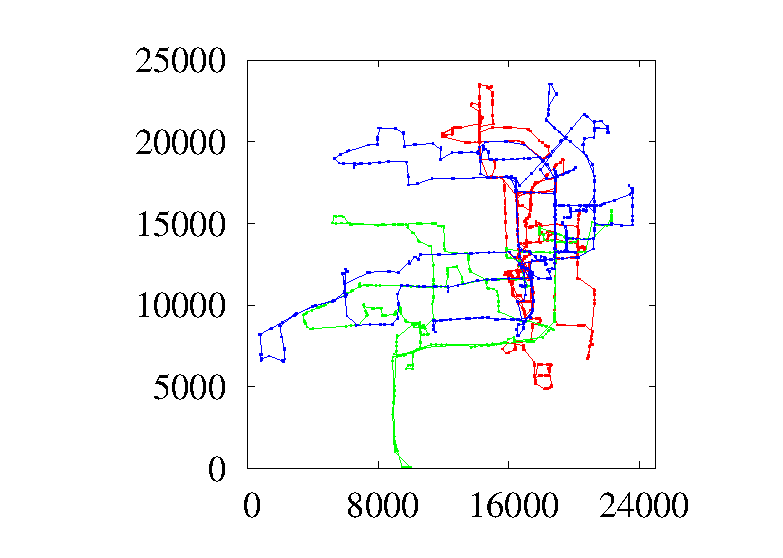
\includegraphics[width=0.24\textwidth]{figures/Evaluation/trace_real.eps}}
\subfigure[START]{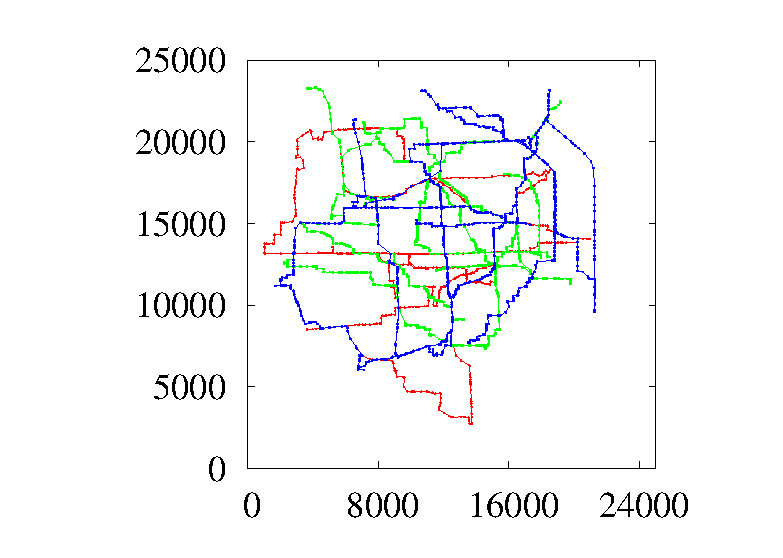
\includegraphics[width=0.24\textwidth]{figures/Evaluation/trace_start.eps}}
\subfigure[SP]{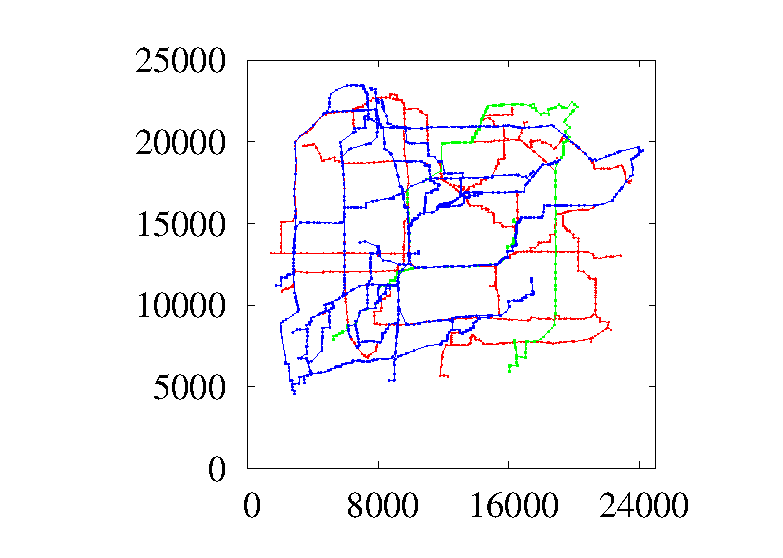
\includegraphics[width=0.24\textwidth]{figures/Evaluation/trace_sp.eps}}
\subfigure[RWP]{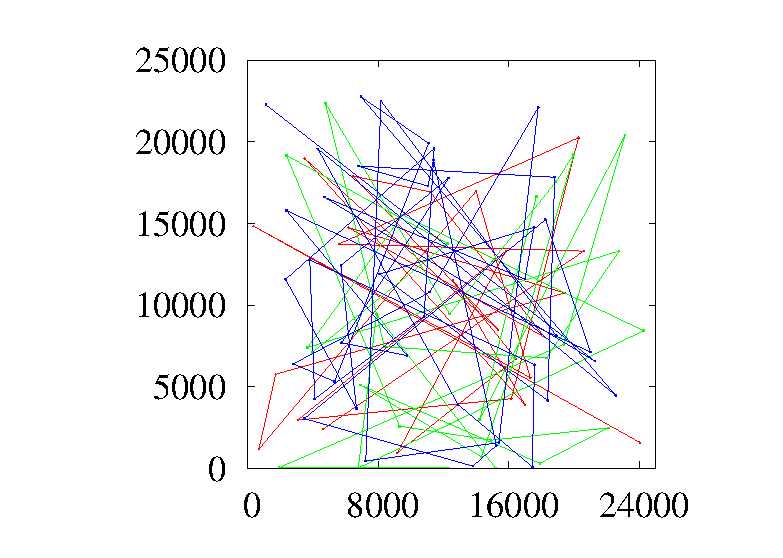
\includegraphics[width=0.24\textwidth]{figures/Evaluation/trace_rwp.eps}}
\caption{Trace samples.}\label{figure_tracesample}
\end{figure*}
\begin{figure*}[!t]
\centering
\subfigure[Real Trace]{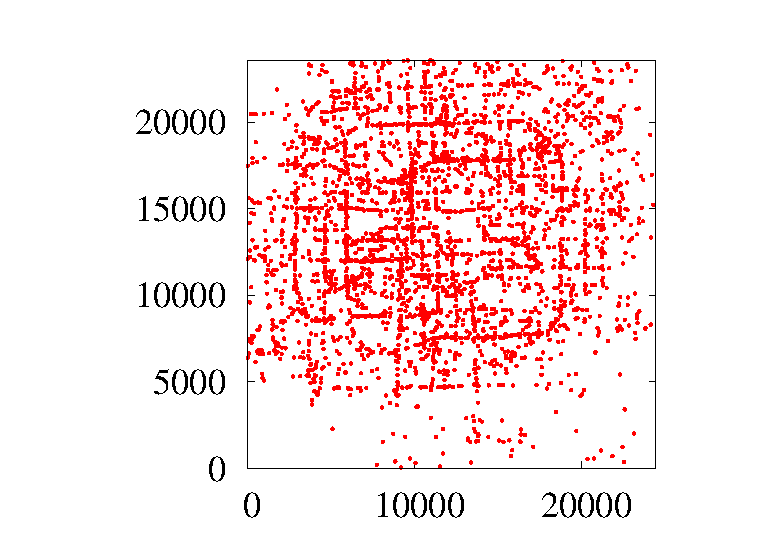
\includegraphics[width=0.24\textwidth]{figures/Evaluation/sample/tracesample.eps}}
\subfigure[START]{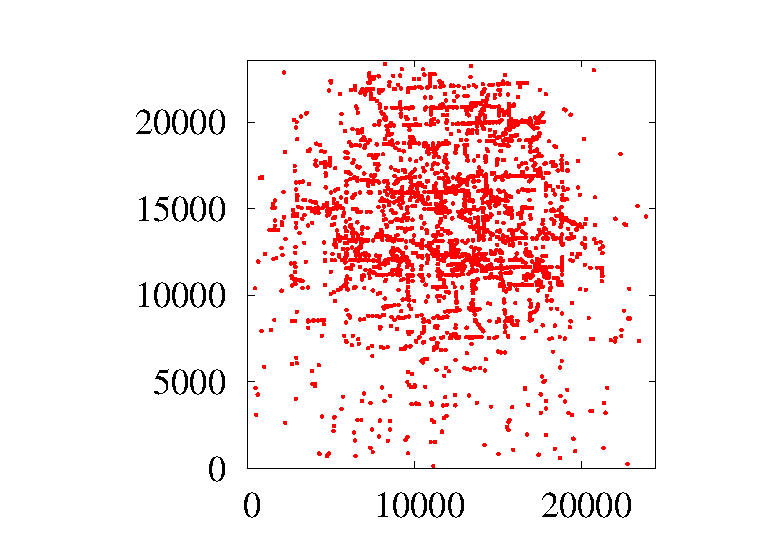
\includegraphics[width=0.24\textwidth]{figures/Evaluation/sample/startsample.eps}}
\subfigure[SP]{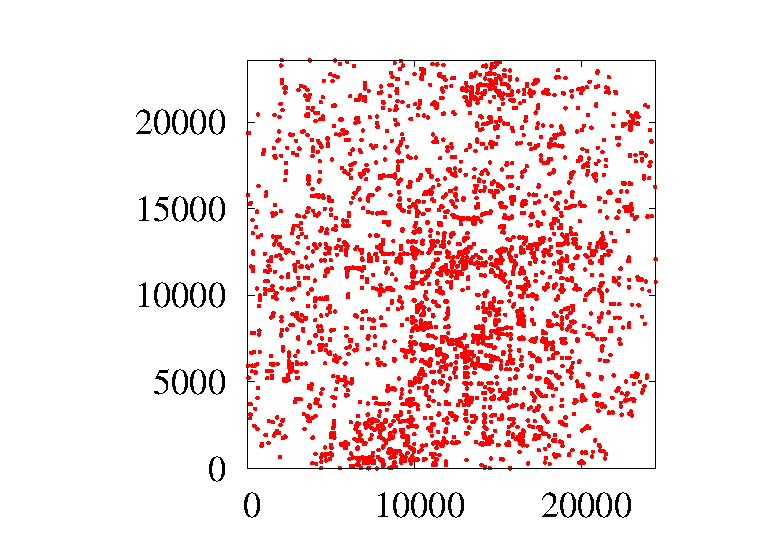
\includegraphics[width=0.24\textwidth]{figures/Evaluation/sample/spsample.eps}}
\subfigure[RWP]{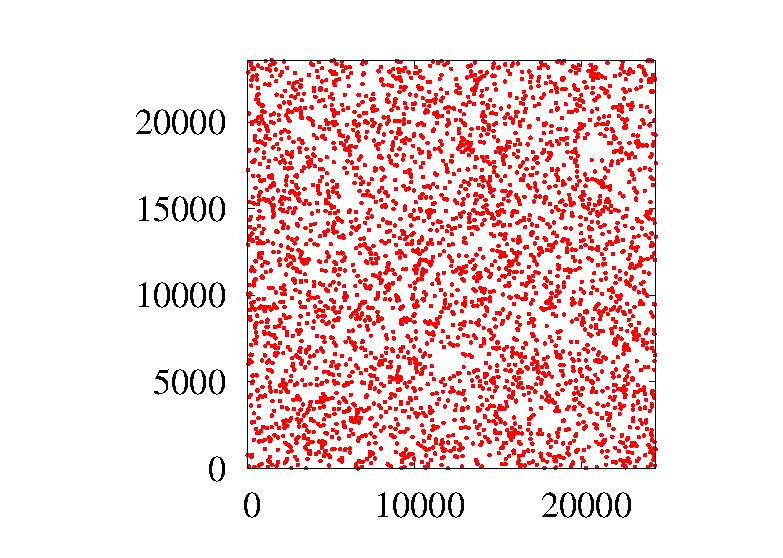
\includegraphics[width=0.24\textwidth]{figures/Evaluation/sample/rwpsample.eps}}
\caption{Trace snapshots.}\label{figure_trace_snapshots}
\end{figure*}

\section{Model Verification}
\label{section_model_varification}
In this section, START mobility model is validated on the aspects of node distribution and contact characteristics compared with existing mobility models and the real traces. We pick two simple mobility models for comparison: one free space - Random Way Point (RWP) model, the other is constrained model, Shortest Path (SP).  SP mobility model is based on the underlying map of Beijing where vehicles move along the map roads by Dijkstra algorithm to random destinations. Both models take no consideration of the node statuses and geographical distributions. All mobility models are implemented on Opportunistic Networking Environment (ONE)\cite{KeranenOtt-155}.

In our simulations, $4,000$ vehicles are deployed in an area of $24,445\times 23,584 m^2$ (a sub-map of the whole area, including fourth ring roads in Beijing). The speed range of RWP and SP need to be configured.
To ensure the accuracy, we choose three different speed ranges $[0,44.4]m/s$, $[0,33.3]m/s$ and $[0,22.2]m/s$ (the upper bounds of speed match the speed limits $80$,$120$,$160$ $km/h$. 
The simulation time is one hours.
In order to evaluate contact characteristics, we should define the transmit ranges.
In our simulations, the transmit ranges of high-speed interfaces and blue tooth interface are both set to $200m$ for potential contacts.
All other settings are left at their default values.

\subsection{Traces and Node Distributions}

Trace samples and their snapshots from different mobility models are reported in Fig.~\ref{figure_tracesample} and Fig~\ref{figure_trace_snapshots}. Fig.~\ref{figure_tracesample} shows the trace in one day. The traces of the real data and START only cover some parts of the area, while the traces of SP and RWP almost go through the whole area. Recall that SP and RWP select a destination randomly in the area, while START takes the associations between current region and destinations into consideration (which satisfies the movement rules of taxis). In Fig.~\ref{figure_trace_snapshots}, real trace, START and SP exhibit the road structures, while the node distribution of RWP is much uniform. As to START, the destination section process decides that it tends to select a destination in the regions with higher load/drop event probability. Therefore, with the decline of the randomness, the snapshot of START becomes much clear and centralized on the main roads, which matches real traces very well.

%\begin{figure}[!h]
%\centering
%\hspace{0.in}
%\subfigure[Real Trace]{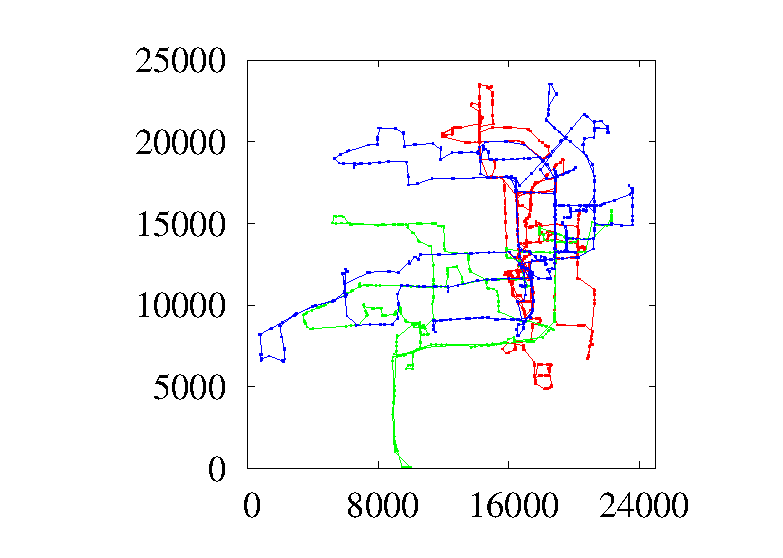
\includegraphics[width=0.23\textwidth]{figures/Evaluation/trace_real.eps}}
%\hspace{0.0in}
%\subfigure[START]{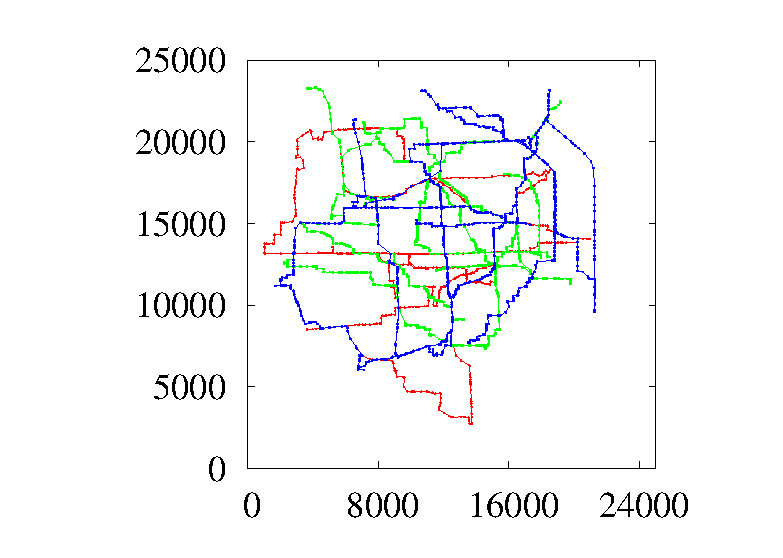
\includegraphics[width=0.23\textwidth]{figures/Evaluation/trace_start.eps}}
%\hspace{0.0in}
%\subfigure[SP]{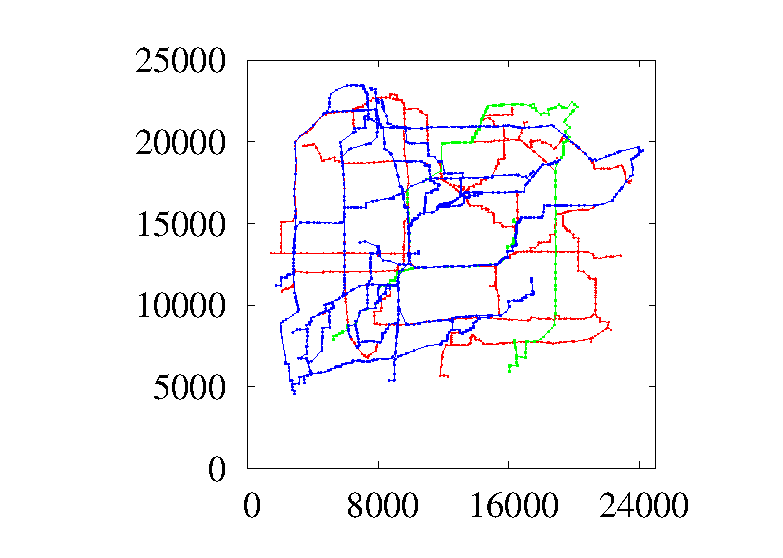
\includegraphics[width=0.23\textwidth]{figures/Evaluation/trace_sp.eps}}
%\hspace{0.in}
%\subfigure[RWP]{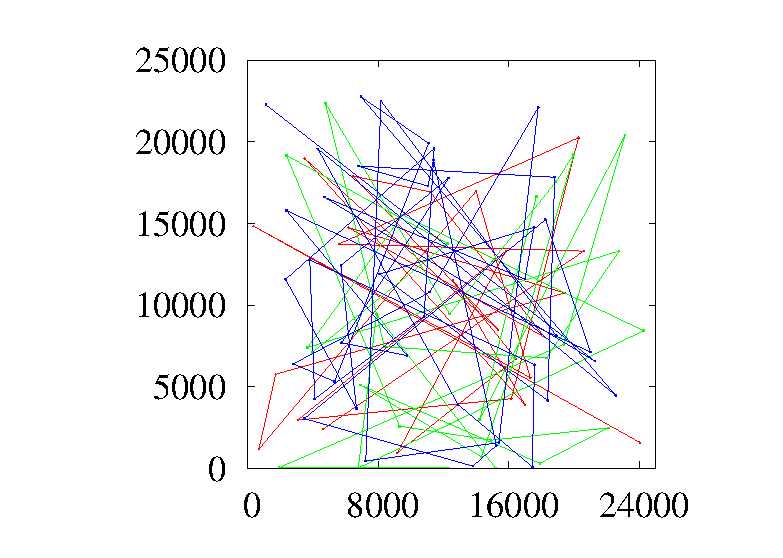
\includegraphics[width=0.23\textwidth]{figures/Evaluation/trace_rwp.eps}}
%\caption{Trace samples}\label{figure_tracesample}
%\end{figure}

%\begin{figure}[!h]
%\centering
%\subfigure[Real Trace]{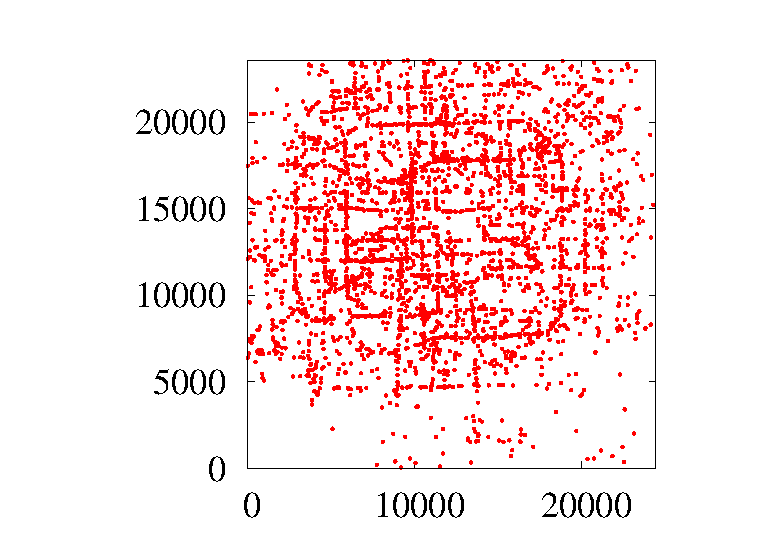
\includegraphics[width=0.23\textwidth]{figures/Evaluation/sample/tracesample.eps}}
%\vspace{0.in}
%\hspace{0.0in}
%\subfigure[START]{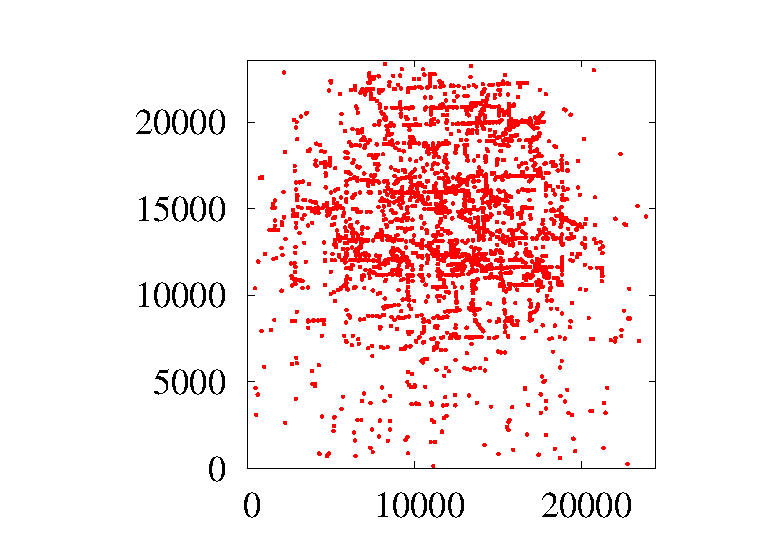
\includegraphics[width=0.23\textwidth]{figures/Evaluation/sample/startsample.eps}}
%\vspace{0.in}
%\hspace{0.0in}
%\subfigure[SP]{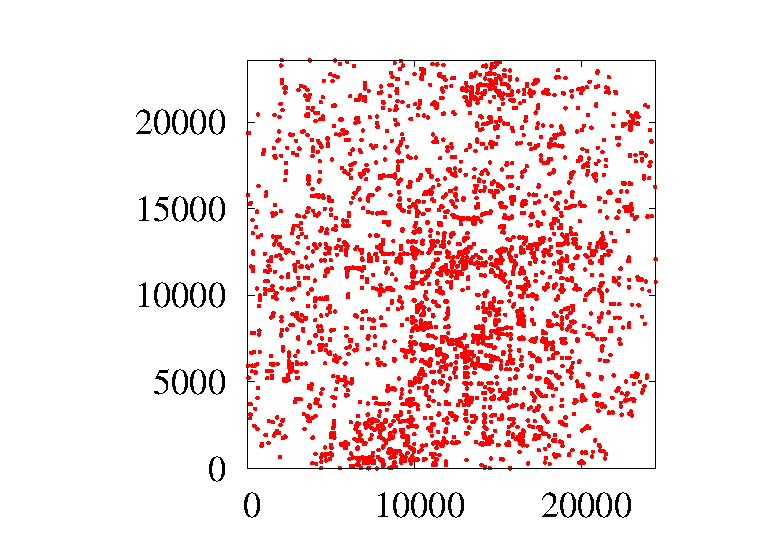
\includegraphics[width=0.23\textwidth]{figures/Evaluation/sample/spsample.eps}}
%\vspace{0.in}
%\hspace{0.0in}
%\subfigure[RWP]{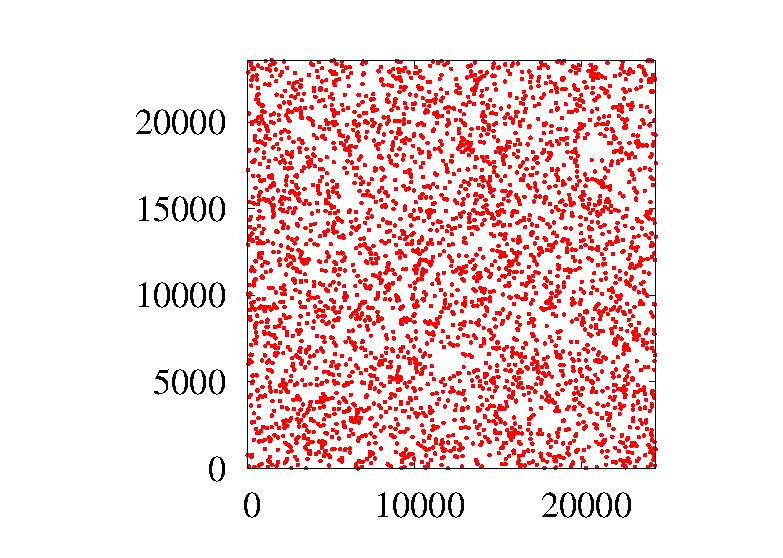
\includegraphics[width=0.23\textwidth]{figures/Evaluation/sample/rwpsample.eps}}
%\caption{Trace snapshots}\label{figure_trace_snapshots}
%\end{figure}

\subsection{Contacts Characteristics}

\begin{figure}[!h]
\centering
\subfigure[cumulative contact time distribution]{
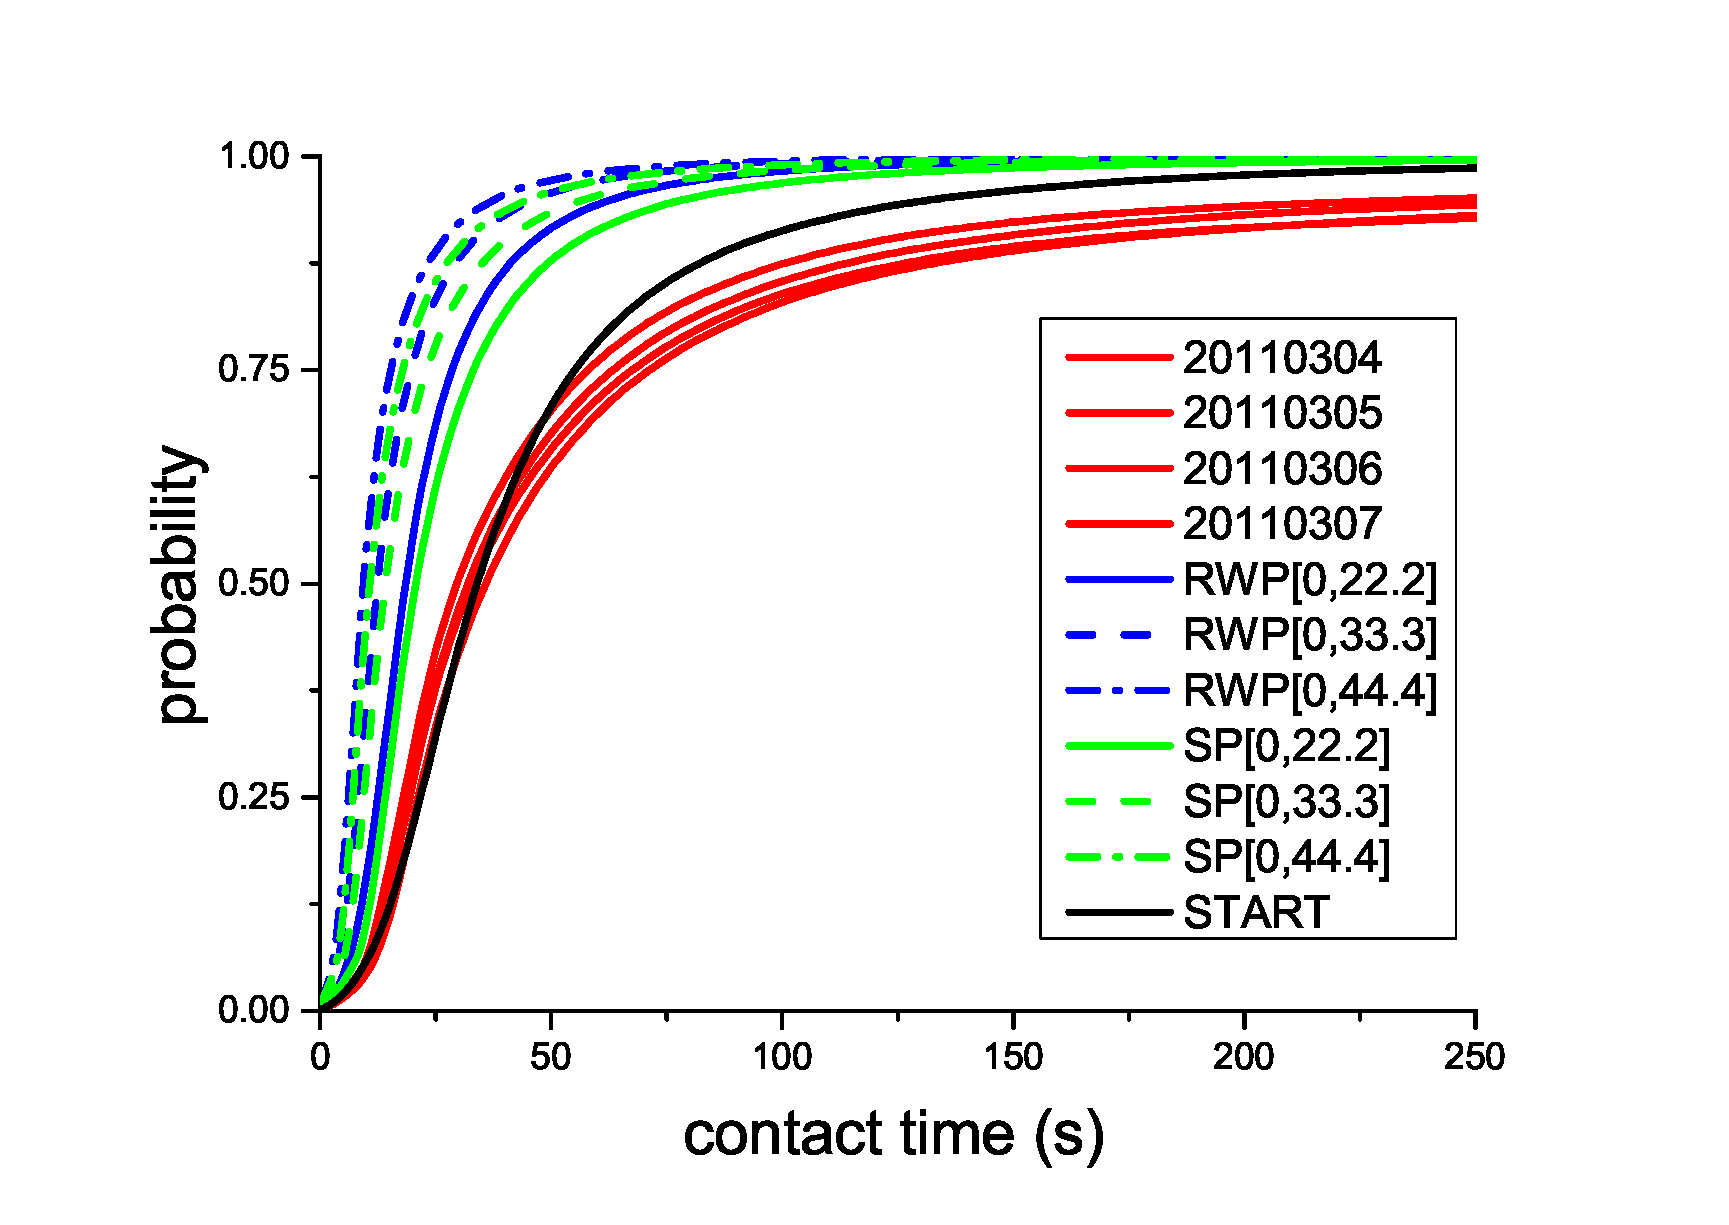
\includegraphics[width=0.4\textwidth]{figures/Evaluation/contact/ct_ccdf.eps}
}
\subfigure[cumulative inter contact time distribution]{
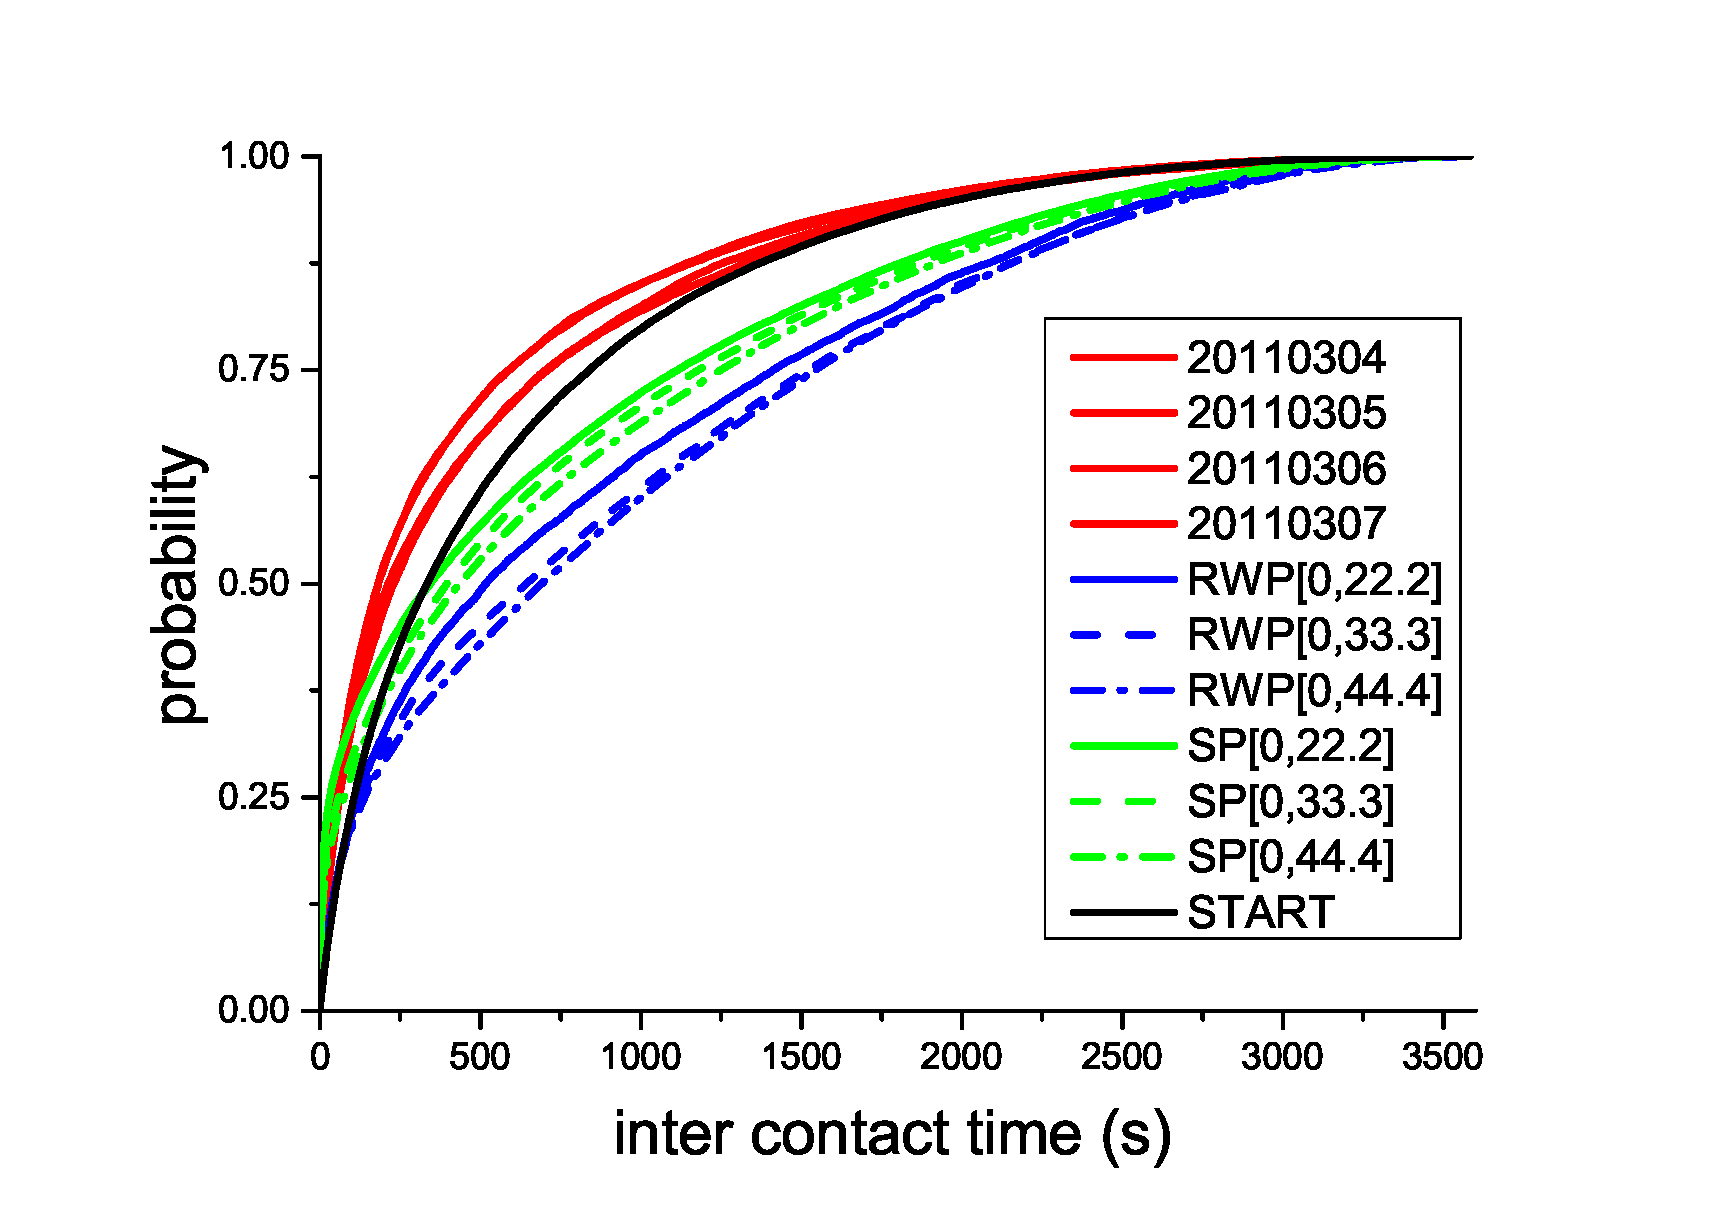
\includegraphics[width=0.4\textwidth]{figures/Evaluation/contact/ict_ccdf.eps}
}
\caption{Contact time, inter contact time distribution.}\label{figure_contacts}
\end{figure}
\begin{figure}[!t]
\centering
\subfigure[time vs. total contact time]{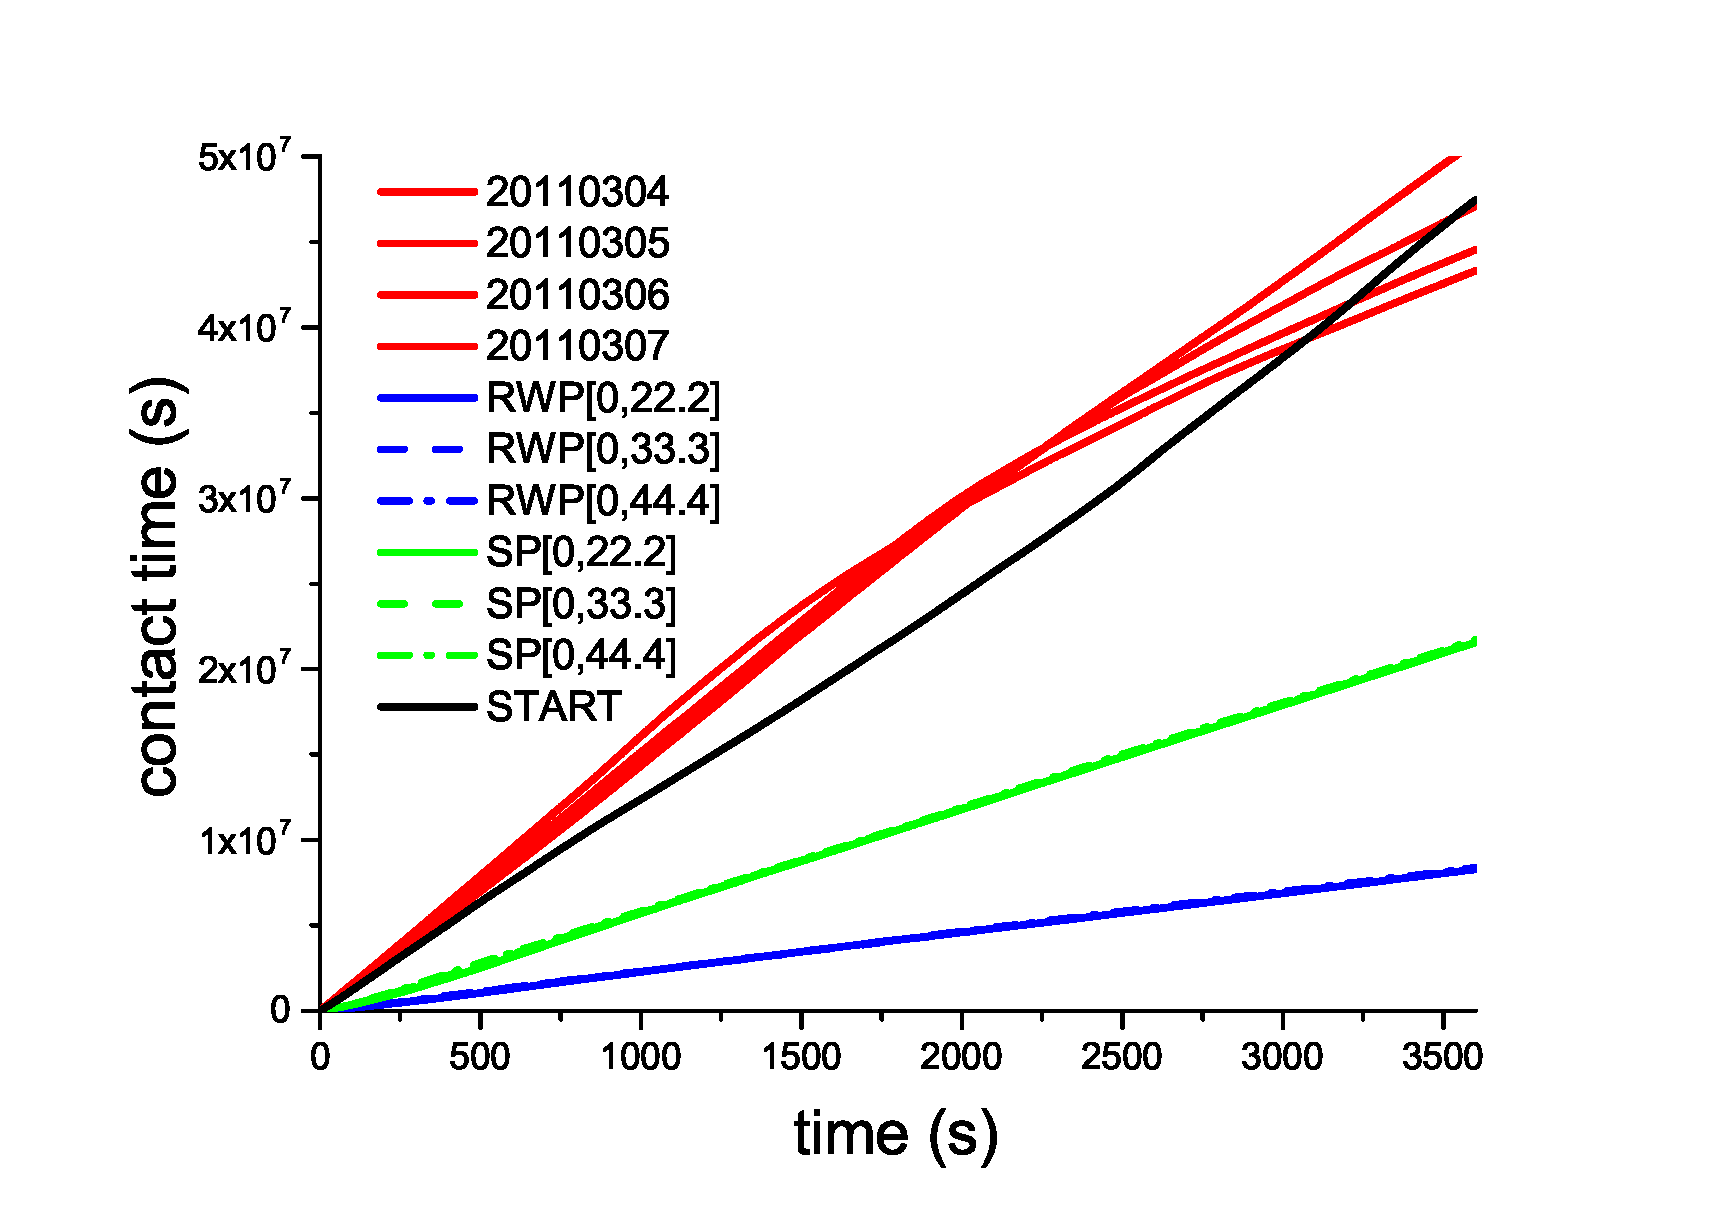
\includegraphics[width=0.4\textwidth]{figures/Evaluation/contact/tc.eps}}
\subfigure[time vs. total contact time in logscale]{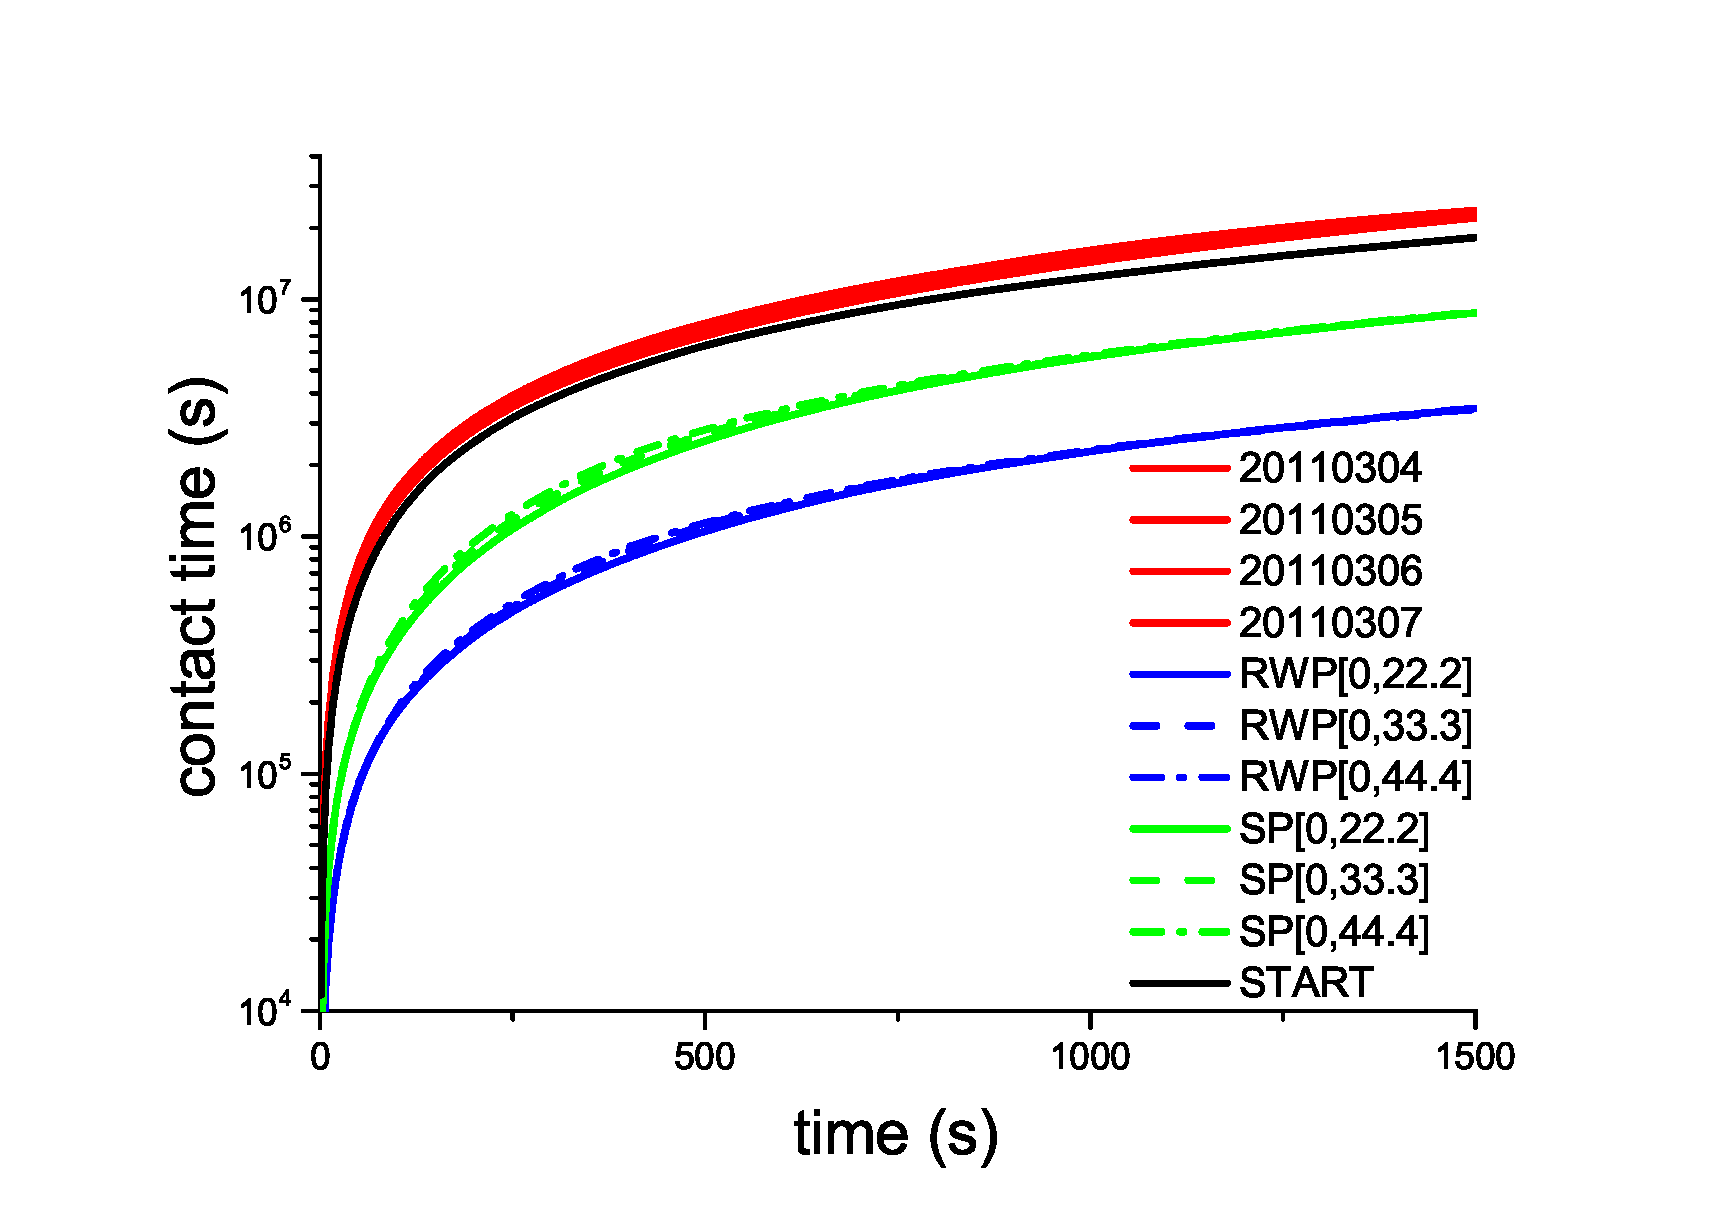
\includegraphics[width=0.4\textwidth]{figures/Evaluation/contact/tc_logscale.eps}}
\caption{Time vs. total contact time.}\label{figure_total_contact_time}
\end{figure}

The contact time and inter contact time among vehicles are also evaluated as the indicators to validate the similarity.
Fig. \ref{figure_contacts} reports the contact time and inter-contact distributions, which shows the probability of the contact or inter-contact time smaller than certain time length. To substantiate, a point $(25,0.5)$ in the plots means the probability is $0.5$ when contact or inter-contact time is shorter than $25s$. Clearly, START matches the real traces best among three mobility models.
Fig. \ref{figure_total_contact_time} also show the sum of contact time regarding to the simulation time.
In Fig. \ref{figure_total_contact_time}(a), the three green lines of SP and the three blue lines of RWP are overlapping with each other.
To recognize the differences, we set y axis as log-scale and set range on x-axis from 0 to 1500 in Fig.~\ref{figure_total_contact_time}(b). The curves of the total contact time vs. time present a liner law. For SP and RWP, the differences of speed ranges show little influence on these curves.
Clearly, the rank of the contact characteristic similarity with the real data is START $>$ SP $>$ RWP.

To conclude, by comparing the node distribution and contact characteristics, the evaluation results confirm that START mobility model achieves great similarities with the real data. START takes the usage of speed and geographic features related with taxi status, while SP employs the map information and RWP is a random model taking use of no realistic data.

